% Figure 2 (text width). File: figures/fig_main_narrowing.pdf from the figures agent (stand-in: narrowing_imbalance.pdf until delivered).
\begin{figure*}[t]
  \centering
  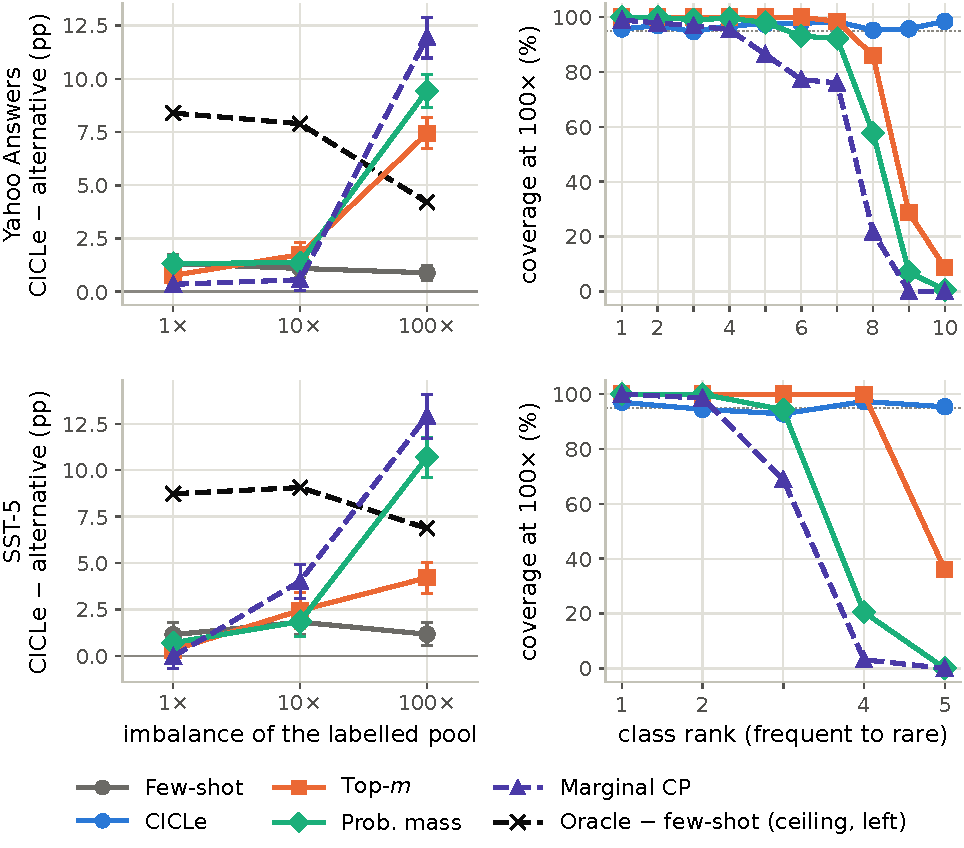
\includegraphics[width=0.85\textwidth]{figures/fig_main_narrowing.pdf}
  \caption{Narrowing rules when the labelled pool is long-tailed, on Yahoo Answers (top) and SST-5 (bottom). The 1,600 training examples are resampled so that the largest class is 1, 10 or 100 times the smallest, while the test sample stays the same. All rules build candidate sets from the same classifier and use the same prompt and Per-Class retrieval. CICLe keeps the classes admitted by class-conditional conformal prediction at $\alpha = 0.05$. Top-$m$ keeps the $m$ most probable classes, with $m$ equal to CICLe's mean set size. Probability mass keeps the most probable classes until their probabilities reach 0.95, and marginal CP uses one conformal threshold for all classes, so these two are not matched in size. (a) CICLe minus each alternative in macro-F1 points, paired over six models, three seeds and $k \in \{1, 4\}$ (36 pairs per point), with 95\% bootstrap intervals over test instances. The dashed line is an oracle set holding the gold label and random classes at CICLe's size, minus few-shot prompting. (b) Coverage of the gold label per class at 100 times imbalance, by frequency rank in the pool, mean over three seeds, with the 95\% target dotted.} % PENDING: size-matched probability-mass and marginal rules
  \label{fig:main_narrowing}
\end{figure*}
